%    This file is part of BGSU.cls The BGSU (Thesis and Dissertation LaTeX class)
%
%    BGSU.cls is free software: you can redistribute it and/or modify
%    it under the terms of the GNU General Public License as published by
%    the Free Software Foundation, either version 3 of the License, or
%    (at your option) any later version.
%
%    BGSU.cls is distributed in the hope that it will be useful,
%    but WITHOUT ANY WARRANTY; without even the implied warranty of
%    MERCHANTABILITY or FITNESS FOR A PARTICULAR PURPOSE.  See the
%    GNU General Public License for more details.
%
%    You should have received a copy of the GNU General Public License
%    along with BGSU.cls  If not, see <http://www.gnu.org/licenses/>.
%
%    Note that this only applies to the example and template files and BGSU.cls
%    itself. Any actual document content (such as your thesis or dissertation text)
%    belongs solely to you and you can do with it what you please.

\documentclass{BGSU}

% For thesis, open BGSU.cls and change line 57 to \def\@doctype{Thesis}

% packages amsmath and amsthm are loaded in BGSU.cls file

\usepackage{amsmath}   % load the AMS math package
\usepackage{amsthm}    % allows AMS definitions for theorems, proofs, etc.
\usepackage{amssymb}   % allows the use of AMS symbols like blackboard bold
\usepackage{graphicx}  % for including graphics files and images
\usepackage{caption}
\captionsetup[table]{labelsep=space}
\captionsetup[figure]{labelsep=space}
\usepackage{epstopdf}
\usepackage{tocloft}
\setlength{\cftbeforetoctitleskip}{-25pt}
\setlength{\cftbeforeloftitleskip}{-25pt}
\setlength{\cftbeforelottitleskip}{-25pt}
\usepackage{times}     % Times New Roman (nimbus version)
\usepackage{listings}  % allows program codes embeded with original forms
\usepackage{bookmark}  % make it possible to add PDF bookmarks at will
\usepackage{pdflscape} % make it possible to use landscape environment
\usepackage[nottoc,notlof,notlot]{tocbibind} % keep list of figures, tables, out of the table of contents, also keep the table of contents out of the table of contents
\usepackage[longnamesfirst]{natbib} %You need to insert comment (%) if you don't want to use natbib for bibliography

% Number theorems, lemmas, etc. together with equation numbers
% This makes things easier to find in the dissertation, a great help to readers

\newtheorem{theorem}[equation]{{\bf Theorem}}
\newtheorem{lemma}[equation]{\bf Lemma}
\newtheorem{remark}[equation]{\bf Remark}
\newtheorem{definition}[equation]{\bf Definition}
\newtheorem{convention}[equation]{\bf Convention}
\newtheorem{proposition}[equation]{\bf Proposition}
\newtheorem{notation}[equation]{\bf Notation}
\newtheorem{corollary}[equation]{\bf Corollary}
\newtheorem{example}[equation]{{\bf Example}}

% Alternatively, number these using the theorem counter
%\newtheorem{theorem}{Theorem}[chapter]         % Allow numbered theorems
%\newtheorem{lemma}[theorem]{\bf Lemma.}
%\newtheorem{remark}[theorem]{\bf Remark.}
%\newtheorem{definition}[theorem]{\bf Definition.}
%\newtheorem{convention}[theorem]{\bf Convention.}
%\newtheorem{proposition}[theorem]{\bf Proposition.}
%\newtheorem{notation}[theorem]{\bf Notation.}
%\newtheorem{corollary}[theorem]{\bf Corollary.}
%\newtheorem{example}[theorem]{{\bf Example.}}

% Change the text below -----------------------------------------------

\title{An example dissertation}
\author{Nate Iverson}
\degree{Doctor of Philosophy}
\date{August 2007}
\advisor{Corneliu Hoffman}
\gfr{Darth Vader} % graduate faculty representative
\committee{Kit Chan \\ \\ Warren McGovern}
\keywords{Algebraic topology; Bayesian analysis; more specific to your research}
\subject{Algebra; statistics; broad terms like this}

\begin{document}

\frontmatter   % makes page #'s lower case roman

\maketitle     % produce the title page using the information above

\copyrightpage % copyrighting your dissertation is optional

\begin{abstract}
Darth Vader:
	There is no escape. Don't make me destroy you.
	pauses Luke, you do not yet realize your importance.
	You have only begun to discover your power. Join me,
	and I will complete your training. With our combined
	strength, we can end this destructive conflict and
	bring order to the galaxy.
Luke Skywalker:
	I'll never join you!
Darth Vader:
	If you only knew the *power* of the dark side. Obi-wan
	never told you what happened to your father.
Luke Skywalker:
	He told me enough! He told me *you* killed him.
Darth Vader:
	No. *I* am your father.














\end{abstract}

% optional section ``Some students choose to personalize their manuscripts
% with an appropriate quotation or illustration''
% formatting and placement is up to you.
\begin{dedication}
\begin{minipage}{5in}
This is the greatest thrill of my life!  I'm king of the world!  Wooo,
wooo!  Wooo, wooo!\\

		-- Homer Simpson\\
		   Bart the Daredevil
\end{minipage}
\end{dedication}

% optional but encouraged section ``as a means to recognize and express
% appreciation to the people who were influential in preparing and completing
% the manuscript''
\begin{acknowledgments}
I would like to acknowledge \ldots\




\end{acknowledgments}

\pdfbookmark[section]{\contentsname}{toc}  % put toc in PDF bookmarks
\tableofcontents
\pagebreak
\pdfbookmark[section]{LIST OF FIGURES}{figures}
\listoffigures
\pagebreak
\pdfbookmark[section]{LIST OF TABLES}{tables}
\listoftables

% preface section is optional
\begin{preface}
\thispagestyle{myheadings}
Blah Blah Blah...
\end{preface}

\mainmatter % starts over page counter and gives regular page numbers

\chapter{\texorpdfstring{MATHEMATICS}{}} %upper case only
\setcounter{equation}{0} \numberwithin{equation}{section}

\section{Small figures}
This section illustrates how to include a small .eps figure.
You can also use .pdf figures.
Run PDFLaTeX to compile the LaTeX source code.

\begin{figure}[h]
\centering
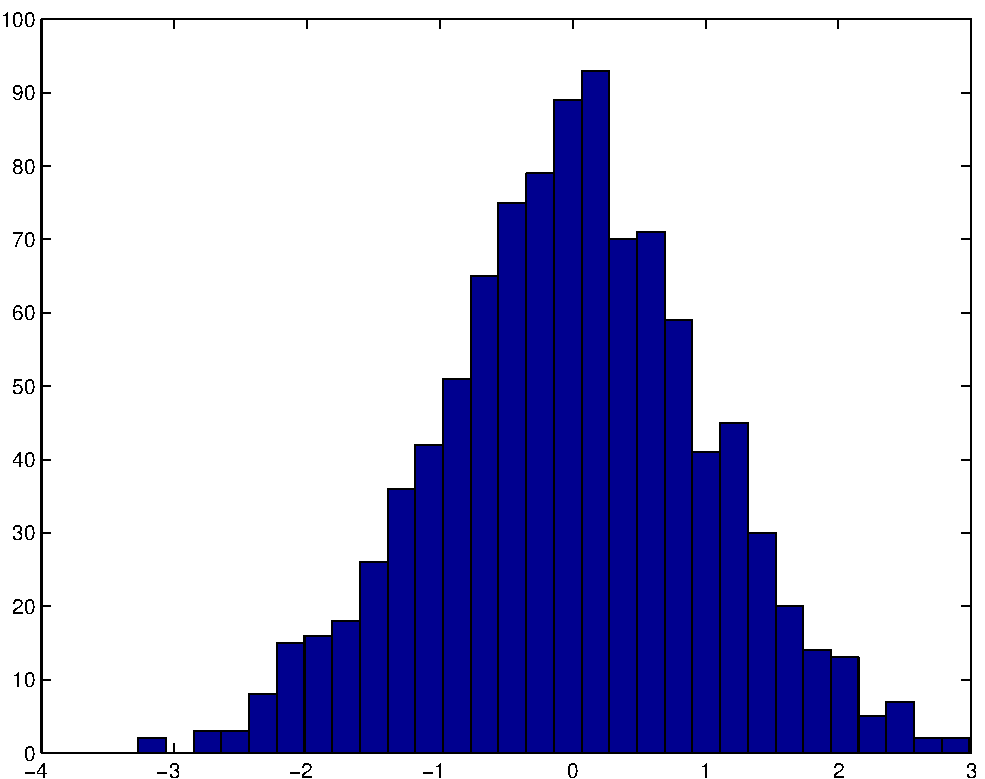
\includegraphics[width = 4.5 in ]{figures/figure-eps-converted-to.pdf}
\caption{Caption of a figure.}\label{FigureLabel}
\end{figure}

\section{Making tables}

\begin{table}[ht]
\centering \caption{The values of test
statistics and the corresponding critical values
at~$t_0.$~~$\alpha=0.1.$~}\label{stanford}\vskip .1in
\begin{tabular}{|c|c|c|c|c|c|c|}\hline
$t_0$ & 30 & 60 & 90 & 120 & 150 & 180 \\ \hline
Critical Value & 11.2282 & 10.5357 & 11.1108 & 11.7942 & 11.7343 & 11.7471\\ \hline
Test Statistic & 25.3182 & 24.6395 & 24.6049 & 25.6623 & 27.1320 & 29.3247\\ \hline
\end{tabular}
\end{table}

\section{Citations}

%If you use the package natbib for citations, here is the example how to cite an article.
%Many thanks to Dr. Maria Rizzo who worked this section.

To cite an article use cite, citet, or citep.

For ``in text'' citations use citet:  The original result is attributed to \citet{vn28}.
Refer to \citet{mardia70} for an example.
Refer to \cite{mardia70} for an example.

For a ``parenthetical citation'' use citep:  The computations were implemented in R \citep{R}
using bootstrap \citep{dh97,et93}.

When citing a book, it is helpful to mention where to find the result by indicating
a chapter or a page number or an equation number:  \citet[Ch.~6]{et93} discuss additional results.

Add your reference information to the file reference.bib.
Every time you edit reference.bib, run BibTeX on the dissertation.tex file so that LaTeX will know what the references are.

%If you don't want to use natbib, you should insert comment (\%) in the above part.  
%Here is the example to cite an article without using natbib package. \cite{forina1991class}

\section{Large, wide figures in landscape orientation}

It's not hard to incorporate very wide figures by making a landscape page in the middle of the PDF.  However, then you need the page number to move, in order to stay in the upper right corner.  That is handled by special LaTeX code in the following example.

\begin{landscape}
\thispagestyle{lscape}
\pagestyle{lscape}
  \begin{figure}
    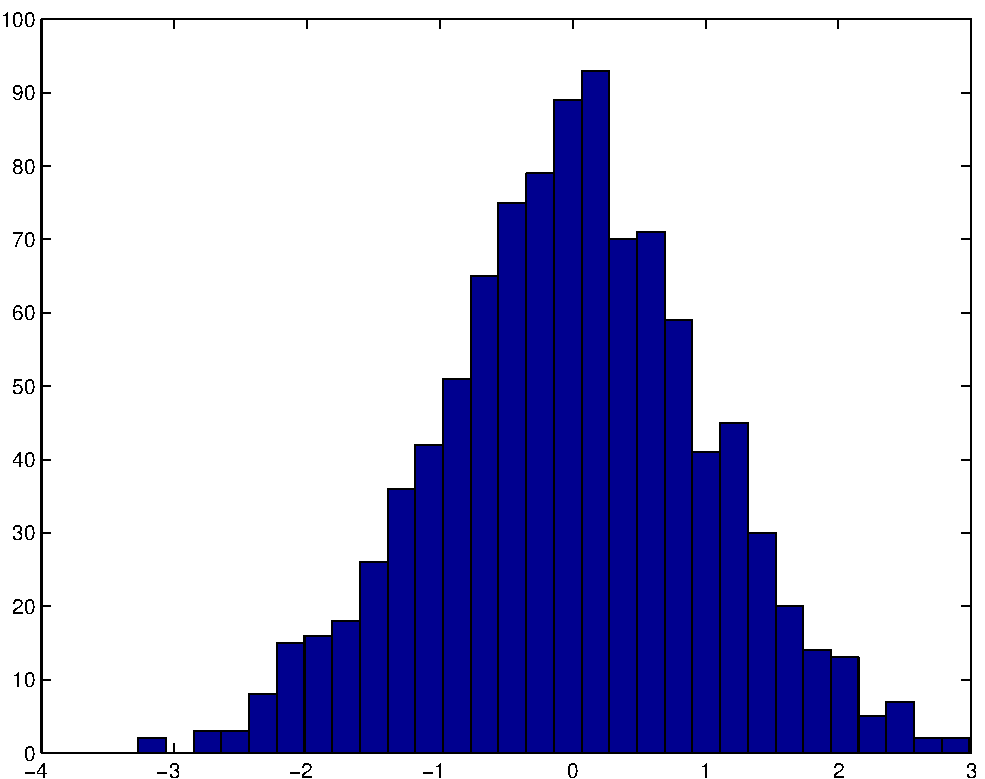
\includegraphics[width=\linewidth,height=\textheight-1in]{figures/figure.pdf}
    \caption[Short caption for List of Figures]{Long caption to appear under the figure.  Make sure the figure is small enough that the caption stays within the margins.  Note that the page number is still in the upper right corner of the PDF file; this is how it needs to be, so follow the code in chapter1.tex.}
  \end{figure}
\end{landscape}

\section{Definitions, Theorems, and proofs}
This section illustrates the normal appearance of definitions, theorems, proofs, and similar items in mathematical work.
Note that these are not listed in a separate list, unlike figures and tables.
All numbered items are counted using the same counter, including equations, theorems, lemmas, etc.
This is not a universal convention in mathematics, but it is super helpful for your readers to be able to find where a theorem or result is.
Also, since we can't have running headers indicating the chapter or section number, these numbers are helpful to indicate to the reader where they are in the document.

\begin{definition}
We say that $\lim_{x \to a} f(x) = L$ if for all $\varepsilon > 0$, there exists $\delta > 0$ such that for all $x \in (a-\delta,a+\delta),$ we have $|f(x) - L| < \varepsilon$.
\end{definition}

\begin{theorem}[Pythagorean Theorem]
For a right triangle with edge lengths $a$, $b$, and $c$ where $c$ is the length of the hypotenuse, 
\begin{equation}
    a^2 + b^2 = c^2
\end{equation}
\end{theorem}
\begin{proof}
Many proofs are available.  Here, we focus on the structure of the proof.

\noindent
{\bf Case 1:} Suppose that the triangle is isosceles.
Then $a = b$ and everything works out well.

\noindent
{\bf Case 2:} Suppose that the triangle is not isosceles.
The proof of this case is beyond the scope of this template.
\end{proof}

\section{Additional numbered results}

\begin{lemma}
A lemma is a short, technical result that is needed in the proof of a theorem.
\end{lemma}

Note how equations are numbered.
\begin{equation}
    (a+b)^2 = a^2 + 2 ab + b^2
\end{equation}

\begin{proposition}
A proposition is like a little theorem.
\end{proposition}

\begin{corollary}
A corollary is an easy result that follows a theorem.
\end{corollary}


\chapter{\texorpdfstring{BOB DYLAN}{}} %upper case only
\setcounter{equation}{0} \numberwithin{equation}{section} 

John the Baptist after poisoning a thief,
Looks up at his hero, the Commander-in-Chief,
Saying tell me great leader, but please make it brief
Is there a hole for me to get sick in?
 The Commander-in-Chief answers him while chasing a fly,
Saying death to all those who would whimper and cry.
And dropping a barbell he points to the sky,
Saying the sun is not yellow, it's chicken.
		-- Bob Dylan, "Tombstone Blues"


\chapter{\texorpdfstring{SILLYNESS}{}} %upper case only
\setcounter{equation}{0} \numberwithin{equation}{section} 

MY NAME IS NOT DR. DEATH\\
MY NAME IS NOT DR. DEATH\\
MY NAME IS NOT DR. DEATH\\
MY NAME IS NOT DR. DEATH\\

	Bart Simpson on chalkboard in episode 8F18

\section{Firefly}
River: "I took you away from there."

Simon: "No."

River: "I know I did. You don't think I do, but... I get confused. I remember
everything. I remember too much and.... Some of it's made up and... some of
it can't be quantified and there's secrets..."

Simon: "It's okay."

River: "But I understand. You gave up everything to find me, and you found me
broken. It's hard for you. You gave up everything you had."

Simon: "Mei mei, everything I have is right here."

\chapter{\texorpdfstring{HOW TO PROVE IT}{}} %upper case only
\setcounter{equation}{0} \numberwithin{equation}{section}

\section{proof by accumulated evidence:}

	Long and diligent search has not revealed a counterexample.

\section{proof by cosmology:}

	The negation of the proposition is unimaginable or
	meaningless. Popular for proofs of the existence of God.

\section{proof by mutual reference:}

	In reference A, Theorem 5 is said to follow from Theorem 3 in
	reference B, which is shown to follow from Corollary 6.2 in
	reference C, which is an easy consequence of Theorem 5 in
	reference A.

\section{proof by metaproof:}

	A method is given to construct the desired proof. The
	correctness of the method is proved by any of these
	techniques.

\chapter{\texorpdfstring{OTHERNESS}{}} %upper case only
\setcounter{equation}{0} \numberwithin{equation}{section}

In a surprise raid last night, federal agents ransacked a house in search
of a rebel computer hacker.  However, they were unable to complete the arrest
because the warrant was made out in the name of Don Provan, while the only
person in the house was named don provan.  Proving, once again, that Unix is
superior to Tops10.

\section{deja-vu}

Over the years, I've developed my sense of deja vu so acutely that now
I can remember things that *have* happened before ...




\backmatter

%bibliography section: there are two options here. 1. Uncomment the following codes and use \bibitem{} to add more articles.
%\begin{thebibliography}{99}
%\bibitem{forina1991class} Forina, M., Armanino, C., Leardi, R., and Drava, G. (1991). A class-modelling technique based on potential functions. \textit{Journal of Chemometrics,} {\textbf{5(5)},} 435-453.
%\end{thebibliography}

%2. Using natbib package (you may use other bibliography types). Refer to http://en.wikibooks.org/wiki/LaTeX/Bibliography_Management
\bibliographystyle{chicago}    %% this one looks best
%\bibliographystyle{apalike}   %% looks okay for dissertations but it puts quotes around titles in references
\setcitestyle{authoryear, open={((},close={))}}
\bibliography{reference}

% appendix section: if you have more than one appendix section, you should use APPENDIX A, APPENDIX B, ....
\mbox{}\newpage
\phantomsection
\appendix
\chapter{\texorpdfstring{APPENDIX A\hspace{1em}SELECTED R PROGRAMS}{APPENDIX A}}

Text of appendix goes here.

% If you want to put program codes in the appendix, here is one example. 
\begin{itemize}
\item The function kernel is used to compute the kernel function of variances
{\small
\begin{lstlisting}
kernel<-function(x,y){
  h <- 0.5*(x-y)^2
  return(h)
}
\end{lstlisting}
}
\end{itemize}

\end{document}
